\documentclass{beamer}
\usetheme{Boadilla}

\usepackage{pgfplots}
\usepackage{tikz}
\pgfplotsset{width=9cm,compat=1.9}
\pgfplotsset{every tick label/.append style={font=\tiny}}

\title{Data Structures and Algorithms}
\subtitle{Software Engineering}
\author{Petko Mitkov}
\institute{Sofia University}
\date{\today}

\begin{document}
 \begin{frame}
\titlepage
\end{frame}

\begin{frame}{Execution times}
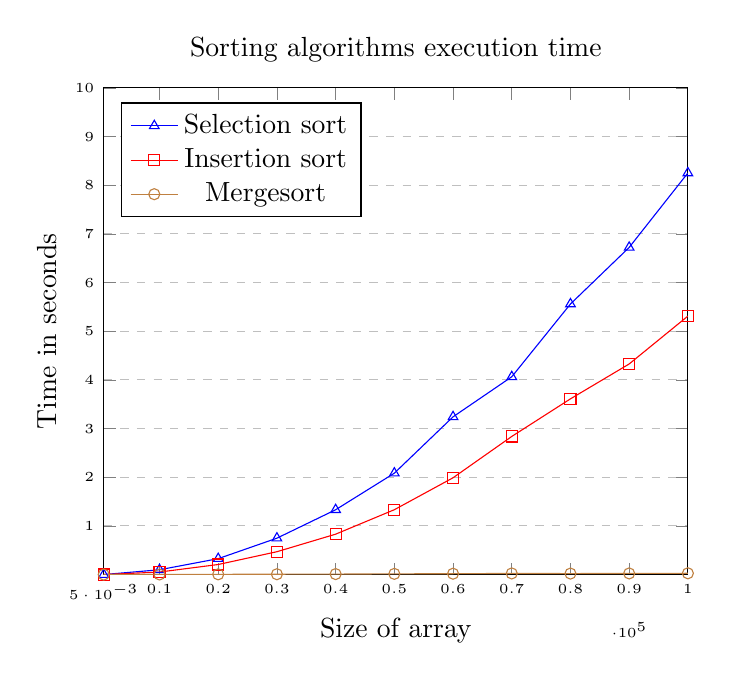
\begin{tikzpicture}
\begin{axis}[
    title={Sorting algorithms execution time},
    xlabel={Size of array},
    ylabel={Time in seconds},
    xmin=500, xmax=100000,
    ymin=0, ymax=10,
    xtick={500, 10000, 20000, 30000, 40000, 50000, 60000, 70000, 80000, 90000, 100000},
    ytick={1,2,3,4,5,6,7,8,9,10},
    legend pos=north west,
    ymajorgrids=true,
    grid style=dashed,
]
 
\addplot[
    color=blue,
    mark=triangle,
    ]
    coordinates {
    (500,0.000326)(10000,0.098745)(20000,0.326853)(30000,0.747888)(40000,1.331735)(50000,2.083295)(60000,3.241116)(70000,4.063787)(80000,5.559606)(90000,6.722031)(100000,8.251414)
    };
    
\addplot[
    color=red,
    mark=square,
    ]
    coordinates {
    (500,0.000189)(10000,0.051861)(20000,0.206798)(30000,0.469638)(40000,0.830098)(50000,1.332527)(60000,1.988821)(70000,2.837740)(80000,3.610519)(90000,4.327234)(100000,5.310966)
    };
    
\addplot[
    color=brown,
    mark=o,
    ]
    coordinates {
    (500,0.000134)(10000,0.002305)(20000,0.004930)(30000,0.007345)(40000,0.009969)(50000,0.014678)(60000,0.017974)(70000,0.023283)(80000,0.020447)(90000,0.023340)(100000,0.026236)
    };
    \legend{Selection sort, Insertion sort, Mergesort}

\end{axis}
\end{tikzpicture}
\end{frame}

\begin{frame}{Execution times}
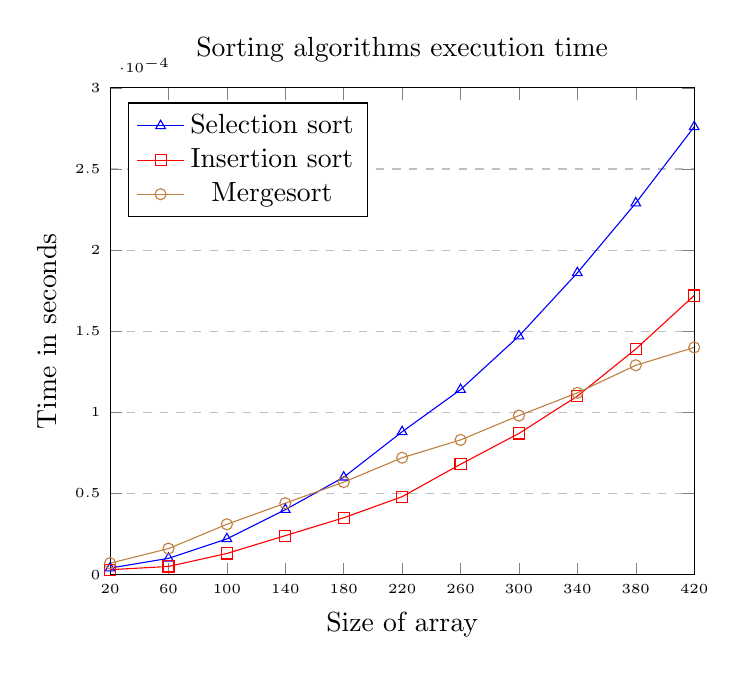
\begin{tikzpicture}
\begin{axis}[
    title={Sorting algorithms execution time},
    xlabel={Size of array},
    ylabel={Time in seconds},
    xmin=20, xmax=420,
    ymin=0, ymax=0.0003,
    xtick={20, 60, 100, 140, 180, 220, 260, 300, 340, 380, 420},
    legend pos=north west,
    ymajorgrids=true,
    grid style=dashed,
]
 
\addplot[
    color=blue,
    mark=triangle,
    ]
    coordinates {
    (20,0.000004)(60,0.000010)(100,0.000022)(140,0.000040)(180,0.000060)(220,0.000088)(260,0.000114)(300,0.000147)(340,0.000186)(380,0.000229)(420,0.000276)
    };
    
\addplot[
    color=red,
    mark=square,
    ]
    coordinates {
    (20,0.000003)(60,0.000005)(100,0.000013)(140,0.000024)(180,0.000035)(220,0.000048)(260,0.000068)(300,0.000087)(340,0.000110)(380,0.000139)(420,0.000172)
    };
    
\addplot[
    color=brown,
    mark=o,
    ]
    coordinates {
    (20,0.000007)(60,0.000016)(100,0.000031)(140,0.000044)(180,0.000057)(220,0.000072)(260,0.000083)(300,0.000098)(340,0.000112)(380,0.000129)(420,0.000140)
    };
    \legend{Selection sort, Insertion sort, Mergesort}

\end{axis}
\end{tikzpicture}
\end{frame}

\end{document}
